\section{Sprint 3: Integracion LLM y n8n}
\label{sec:integracion-llm-n8n}

Con el sprint 2 terminada y viendo que las limitaciones eran evidentes, se tomó la decisión de realizar un cambio fundamental para el futuro del proyecto. Se abandonó 
la idea del sistema de reglas, aunque no en la totalidad, ya que algunas partes nos seguirían siendo útiles. Se decidió integrar un
modelo de lenguaje (LLM) como núcleo o motor del análisis y generación de las páginas. Hasta este momento el sistema intentaba entender los datos mediante
puntuaciones y comparaciones. A partir de este punto, se decidió que fuese la Inteligencia Artificial la encargada de escoger y proponer la estructura del sitio y decidiera que 
campos mostrar. Como se comentó anteriormente, no todo el flujo de análisis e ingesta se cambió, se eliminaron las partes de score y propuesta de dataset, pero el parseo 
y análisis de los campos se mantuvo y modificó levemente, se introdujo todo el dataset en una estructura, que sería la que se pasaría al LLM, de forma que evitaríamos
alucinaciones o errores del LLM en la lectura de la API, obteniendo de esta forma un schema más consistente. Este proceso se describe con más detalle en la subsección~\ref{subsec:proteccion-anti-alucionaciones}


\subsection{Conexión con LLM}
\label{subsec:conexion-llm}

Para poder realizar la conexión con el LLM, el primer paso fue crear el módulo \textbf{utils/llm}, y dentro se creó el archivo \texttt{client.py}, el cual
implementa la función \texttt{chat\_completions}. Esta función se encarga de hacer una única cosa: enviar un mensaje al LLM y devolver la respuesta en texto
plano.

Una decisión importante fue utilizar el estándar de la mayoría de proveedores para realizar la conexión, utilizando de esta forma el endpoint \textbf{/chat/completions}. En este caso creado para poder realizar pruebas con varios LLM de diferentes proveedores (OpenRouter, Groq, NVIDIA) y cualquier agente local.
Otra decisión fue crear \texttt{.env}, de forma que la URL base, la API key y el modelo se leen de variables de entorno definidas en dicho fichero, lo que permite cambiar de proveedor sin tocar una sola línea de código.

La función mencionada anteriormente acepta tres parámetros principales:

\begin{itemize}
    \item \textbf{Mensaje de usuario}: la tarea concreta que se le envía al modelo 
    en cada llamada, en este caso el prompt con los datos del dataset, las claves 
    disponibles y los ejemplos de items reales.
    
    \item \textbf{Mensaje de sistema}: instrucciones previas que definen cómo debe 
    comportarse el modelo antes de procesar el mensaje del usuario. Se utiliza para 
    indicarle el rol que debe adoptar, el formato de respuesta esperado y lo que 
    está prohibido hacer. Es opcional, ya que técnicamente todo puede ir en el 
    mensaje de usuario, pero separarlo es una buena práctica que facilita reutilizar 
    el mismo comportamiento base en distintas llamadas. Por ejemplo, el mensaje de sistema del planner indica al modelo que es un experto en diseño 
    de sitios web, que debe devolver únicamente un objeto JSON válido y que está 
    prohibido inventar campos que no existan en el dataset proporcionado.
    
    \item \textbf{Temperatura}: parámetro que controla el grado de aleatoriedad 
    en las respuestas del modelo. Un valor cercano a 0 produce respuestas más 
    deterministas y predecibles, mientras que valores más altos generan respuestas 
    más creativas pero menos consistentes. En este caso se fija por defecto en 
    \texttt{0.2}, favoreciendo la estabilidad especialmente cuando se espera JSON 
    estructurado como salida.
\end{itemize}

El primer proveedor utilizado fue OpenRouter, con el modelo de meta-llama: \\
\texttt{llama-3.3-70b-instruct:free}, de acceso gratuito y potencia más que suficiente para las primeras pruebas.

% Meter captura de ejemplo de prompt

\begin{figure}[H]
    \centering
    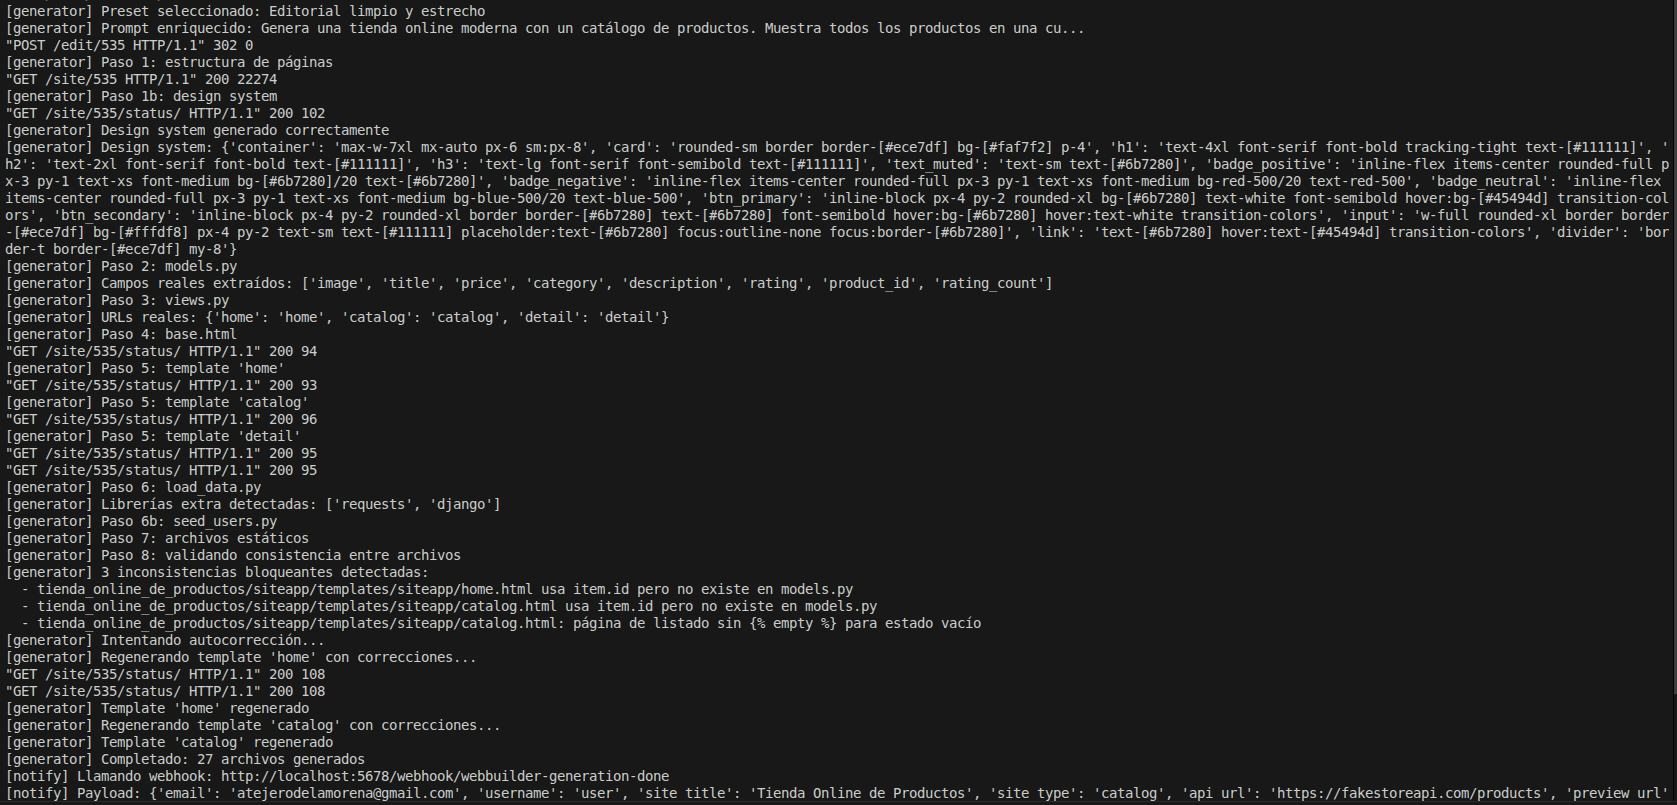
\includegraphics[width=1\textwidth]{img/webbuilder/disenoimplementacion/logs-generacion.png}
    \caption{Ejemplo logs de generación de proyecto}
    \label{fig:Ejemplo logs de generacion}
\end{figure}

\subsection{Planner schema}
\label{subsec:planner-schema}

Otro fichero clave fue \texttt{utils/llm/planner.py} y su función \texttt{generate\_site\_plan}. La misión era transformar el resultado del análisis en un propuesta con campos
concretos de schema que el usuario pudiese aceptar y modificar a su gusto antes de continuar.

El schema tiene una forma fija que el resto del sistema espera:
\begin{itemize}
    \item \textbf{site\_type}: tipo de sitio recomendado, entre \texttt{blog}, \texttt{portfolio}, \texttt{catalog}, \texttt{dashboard} u \texttt{other}.
    \item \textbf{site\_title}: nombre descriptivo del sitio propuesto por el modelo.
    \item \textbf{fields}: lista ordenada de campos del dataset que el sitio debe mostrar, cada uno con su clave original y una etiqueta legible para el usuario.
\end{itemize}

Para obtener este esquema, se construye un prompt estructurado que se envía al LLM. Este prompt es el resultado de una serie de pruebas con distintas formulaciones,  
siguiendo técnicas de \emph{prompt engineering}~\cite{openai_prompt_engineering} para conseguir respuestas consistentes y parseables. La información contenida en este 
prompt es la siguiente:

\begin{itemize}
    \item \textbf{Objetivo del usuario}: texto en lenguaje natural introducido por 
    el usuario describiendo qué tipo de sitio quiere construir.
    
    \item \textbf{Claves disponibles}: lista de campos reales extraídos del dataset 
    durante la fase de análisis. El modelo solo puede proponer campos que estén 
    en esta lista.
    
    \item \textbf{Ejemplos del dataset}: hasta tres items reales del dataset, para 
    que el modelo pueda entender qué tipo de valores contiene cada campo y proponer 
    etiquetas adecuadas.
    
    \item \textbf{Contrato JSON}: estructura exacta que debe devolver el modelo, 
    con los campos obligatorios y su formato esperado.
    
    \item \textbf{Reglas de formato}: conjunto de instrucciones explícitas que 
    indican al modelo que debe devolver únicamente un objeto JSON válido, sin 
    bloques de código Markdown, sin texto introductorio y sin ningún contenido 
    fuera del JSON.
\end{itemize}

Esta rigidez sobre el formato de salida es intencionada, ya que tras la 
realización de varias pruebas, los fallos generados por los diferentes LLM 
siempre eran parecidos. Como esa respuesta se usa directamente en el sistema, 
cualquier texto adicional rompe el proceso de parseo.

De todas formas, debido a las alucinaciones de algunos modelos y a que en 
ocasiones ignoraban las restricciones de formato, se aplicaba una limpieza 
previa sobre la respuesta antes de parsearla. Esta limpieza eliminaba bloques 
de código Markdown como \texttt{```json} o \texttt{```}, que algunos modelos 
añaden automáticamente alrededor del JSON aunque se les indique explícitamente 
que no lo hagan, así como espacios y caracteres sobrantes al inicio y al final 
de la respuesta, los cuales rompían el flujo de ejecución del proyecto.


\begin{figure}[H]
    \centering
    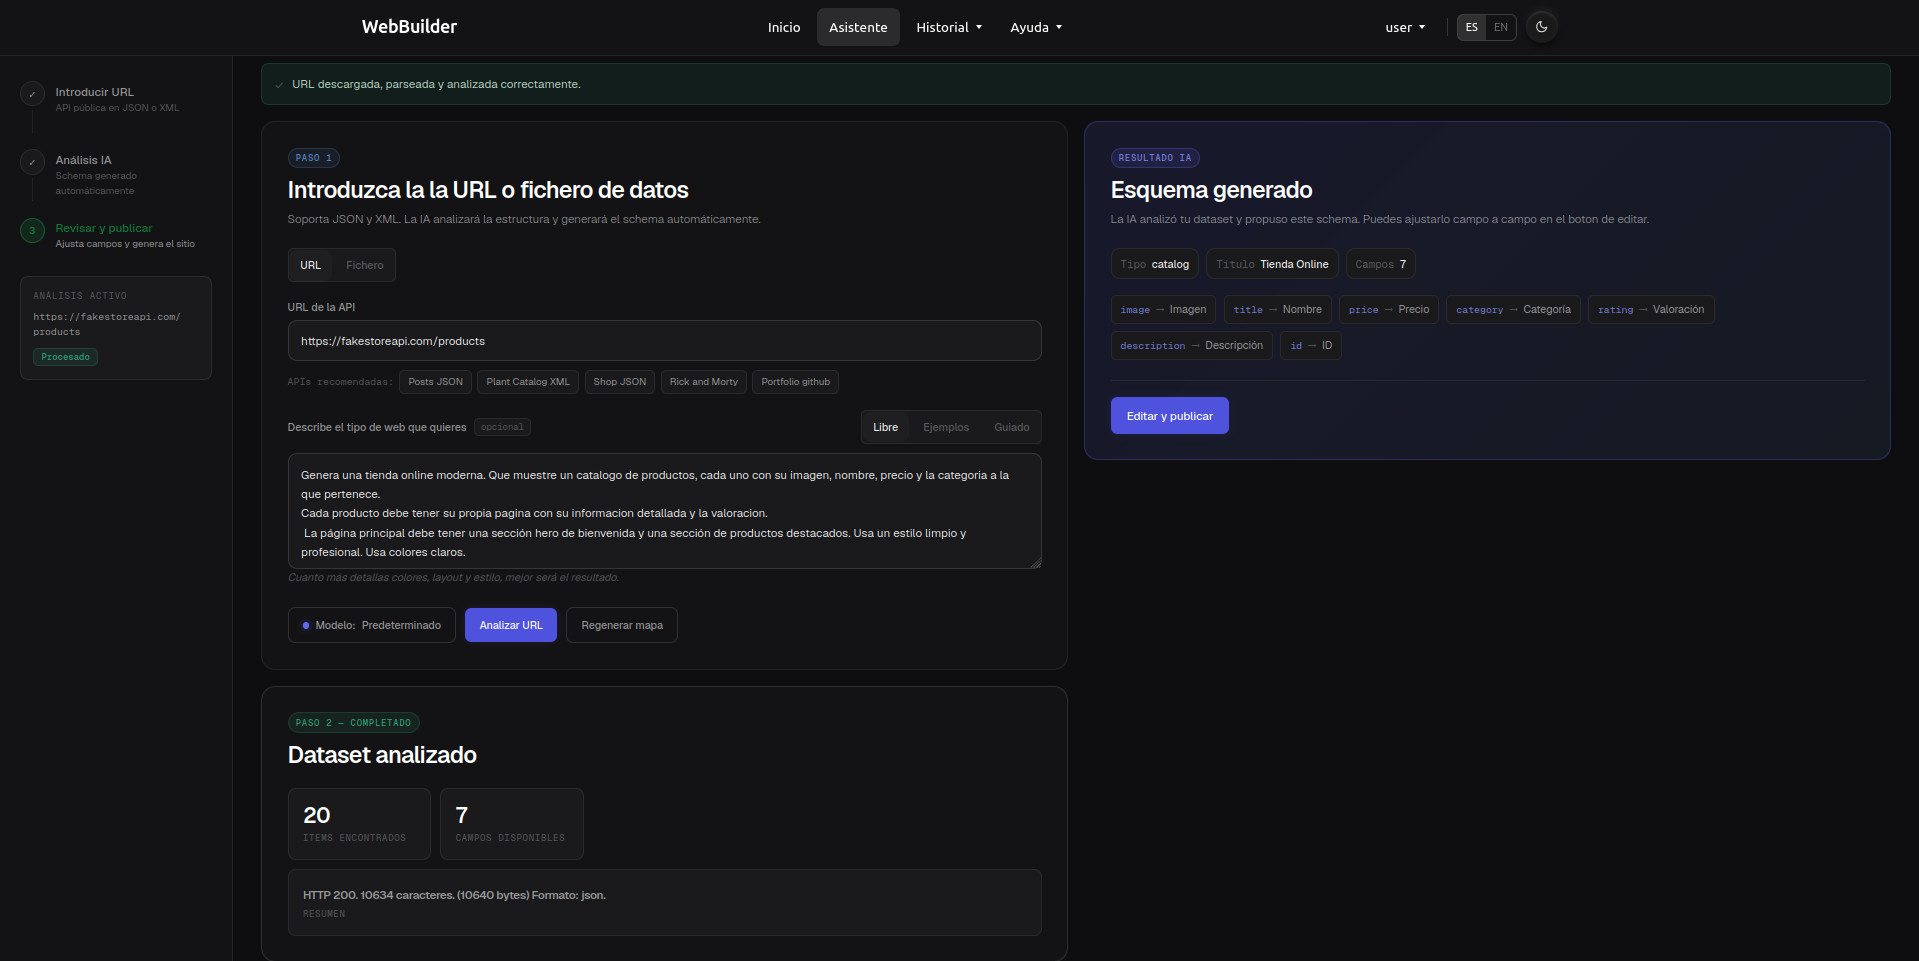
\includegraphics[width=\textwidth]{img/webbuilder/disenoimplementacion/asistente-schema.png}
    \caption{Schema generado automáticamente por el LLM a partir de la API analizada}
    \label{fig:asistente-schema}
\end{figure}

\subsection{Protección anti-alucinaciones}
\label{subsec:proteccion-anti-alucionaciones}

Los errores más comunes siempre sucedían por la misma causa, las alucinaciones del LLM. El error más común era inventar información que no existía en la API, y que nunca se parseo, por lo que no existe en el dataset construido. Para ello hubo que aplicar varias capas de defensa contra alucinaciones para proteger los schemas.

\begin{itemize}
    \item \textbf{Validación contra claves reales}: cada clave propuesta por el LLM se comprueba contra la lista de claves reales extraída del dataset. Si la clave no existe, se intenta un match sin distinguir mayúsculas y minúsculas. Si tampoco hay coincidencia, la clave se descarta silenciosamente.

    \item \textbf{Filtro de tokens prohibidos}: existe una lista de palabras que 
    el modelo confunde con claves del dataset porque forman parte del propio prompt del usuario. 
    Al estar palabras como \texttt{available\_keys}, \texttt{fields} o 
    \texttt{examples} presentes en el texto del prompt, algunos modelos las 
    interpretan erróneamente como campos reales del dataset y las incluyen en su 
    respuesta. Por ejemplo, si el prompt contiene la línea 
    \texttt{"available\_keys": ["name", "date", "url"]}, el modelo puede devolver 
    \texttt{available\_keys} como uno de los campos seleccionados, cuando en 
    realidad es una etiqueta del propio prompt. Cualquier clave que coincida con 
    esta lista se descarta automáticamente.
    
    \item \textbf{Detección de valores disfrazados de claves}: se detectan los 
    casos en los que el modelo introduce un valor concreto del dataset donde 
    debería haber puesto el nombre de un campo. Por ejemplo, si el dataset tiene 
    un campo de fecha, el modelo puede devolver \texttt{2024-01-15} como clave 
    en lugar de \texttt{published\_at}. Para evitarlo, se descartan 
    automáticamente cadenas que sean fechas en formato ISO, URLs completas, 
    extensiones de imagen, valores nulos o texto excesivamente largo.
    
    \item \textbf{Fallback}: si tras aplicar todas las validaciones no queda ninguna clave válida, el sistema construye automáticamente un schema de emergencia con las primeras claves del dataset, garantizando que el flujo nunca se bloquea por un fallo del modelo.
\end{itemize}

Si el parseo falla, el sistema reintenta automáticamente una vez con una pista sobre el error cometido. Si el segundo intento también falla, se activa el fallback. En la Figura~\ref{fig:flujo-url-schema} se muestra el flujo completo desde que el usuario introduce la URL hasta obtener el schema validado.

\begin{figure}[H]
    \centering
    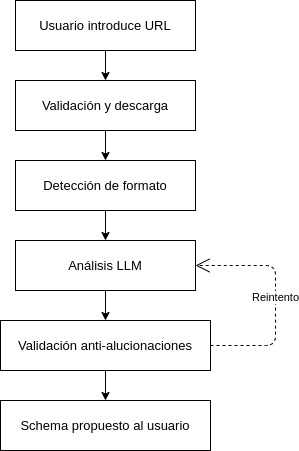
\includegraphics[width=0.4\textwidth]{img/disenoimplementacion/flujourlfase3}
    \caption{Flujo de ingestión y análisis}
    \label{fig:flujo-url-schema}
\end{figure}

\subsection{Actualización de modelos}
\label{subsec:actualizacion-modelos}

La integración del LLM trajo consigo dos cambios importantes.

El primero de ellos fue una modificación en el modelo existente \textbf{APIRequest}, añadiéndole el campo \texttt{plan\_accepted}. Siendo este un booleano encargado de guardar
si el usuario ha aceptado el schema propuesto antes de continuar.

El segundo fue la creación de un nuevo modelo \textbf{GeneratedSite}, 
vinculado con el modelo \texttt{APIRequest} mediante una relación 
\texttt{OneToOne}. Sus campos principales se muestran en la 
Tabla~\ref{tab:modelo-generatedsite}.

\begin{table}[H]
    \centering
    \begin{tabular}{|l|l|p{8cm}|}
        \hline
        \textbf{Campo} & \textbf{Tipo} & \textbf{Descripción} \\
        \hline
        api\_request & OneToOneField & Referencia al análisis que originó el sitio \\
        \hline
        public\_id & UUIDField & Identificador único público del sitio generado \\
        \hline
        plan & JSONField & Schema aceptado por el usuario con los campos seleccionados \\
        \hline
        project\_files & JSONField & Ficheros del proyecto generado indexados por ruta \\
        \hline
    \end{tabular}
    \caption{Campos principales del modelo GeneratedSite en el sprint 3}
    \label{tab:modelo-generatedsite}
\end{table}

\subsection{Integración de n8n}
\label{subsec:integracion-n8n}

En paralelo a la integración del LLM, durante este sprint se incorporó n8n al sistema por primera vez. Es una herramienta de automatización de flujos que permite conectar servicios mediante webhooks y nodos, y que más adelante sería una pieza fundamental de la arquitectura del proyecto. En este momento su uso fue todavía inicial: instalar el entorno y crear el primer flujo de pruebas.

n8n se instaló en un contenedor Docker siguiendo la imagen oficial, quedando disponible en \texttt{localhost:5678}. Una vez levantado el entorno, se creó el primer flujo en n8n y se configuró el primer webhook, apuntando a la ruta \texttt{/webhook-test/WebBuilder-Register}. El prefijo \texttt{webhook-test} indica que el webhook estaba en modo de prueba, el modo que n8n ofrece para verificar que el flujo funciona correctamente antes de activarlo en producción.

La integración en Django se realizó en \texttt{views/auth.py}, donde se añadió la función\texttt{llamar\_webhook}. El nodo se encargaría de notificar a los usuarios recién registrados: Django realizaba una llamada POST a ese webhook con el nombre de usuario y el email del recién registrado, y n8n enviaba automáticamente un correo de bienvenida 
personalizado a esa dirección. Más adelante se completaría el flujo con el webhook de login.

La función estaba diseñada para ser completamente transparente al flujo principal: si n8n no estaba disponible o la llamada fallaba, la excepción se capturaba silenciosamente y el registro continuaba con normalidad. Esto garantizaba que un fallo en el sistema de notificaciones nunca pudiera bloquear el acceso a la aplicación.


\begin{figure}[H]
    \centering
    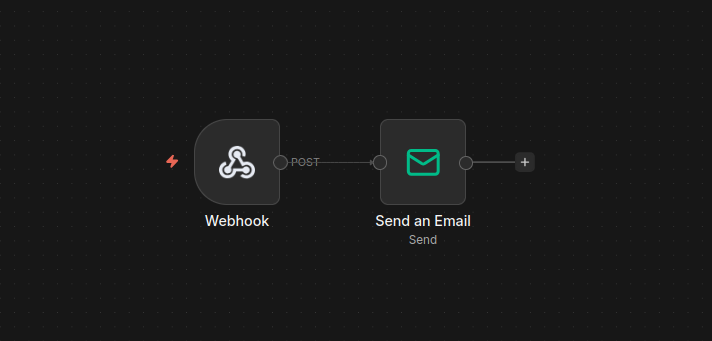
\includegraphics[width=0.7\textwidth]{img/n8n/login-register.png}
    \caption{Flujo n8n login y register}
    \label{fig:Flujo n8n login y register}
\end{figure}